
\begin{table}[H]
    \caption{Mean percentage of pixels per selected SCL class $\pm$ standard deviation derived from 300 MC realizations for all 33 S2 scenes. The overall number of pixels per scene is 360000 (20 $\times$ 20 m spatial resolution).}
    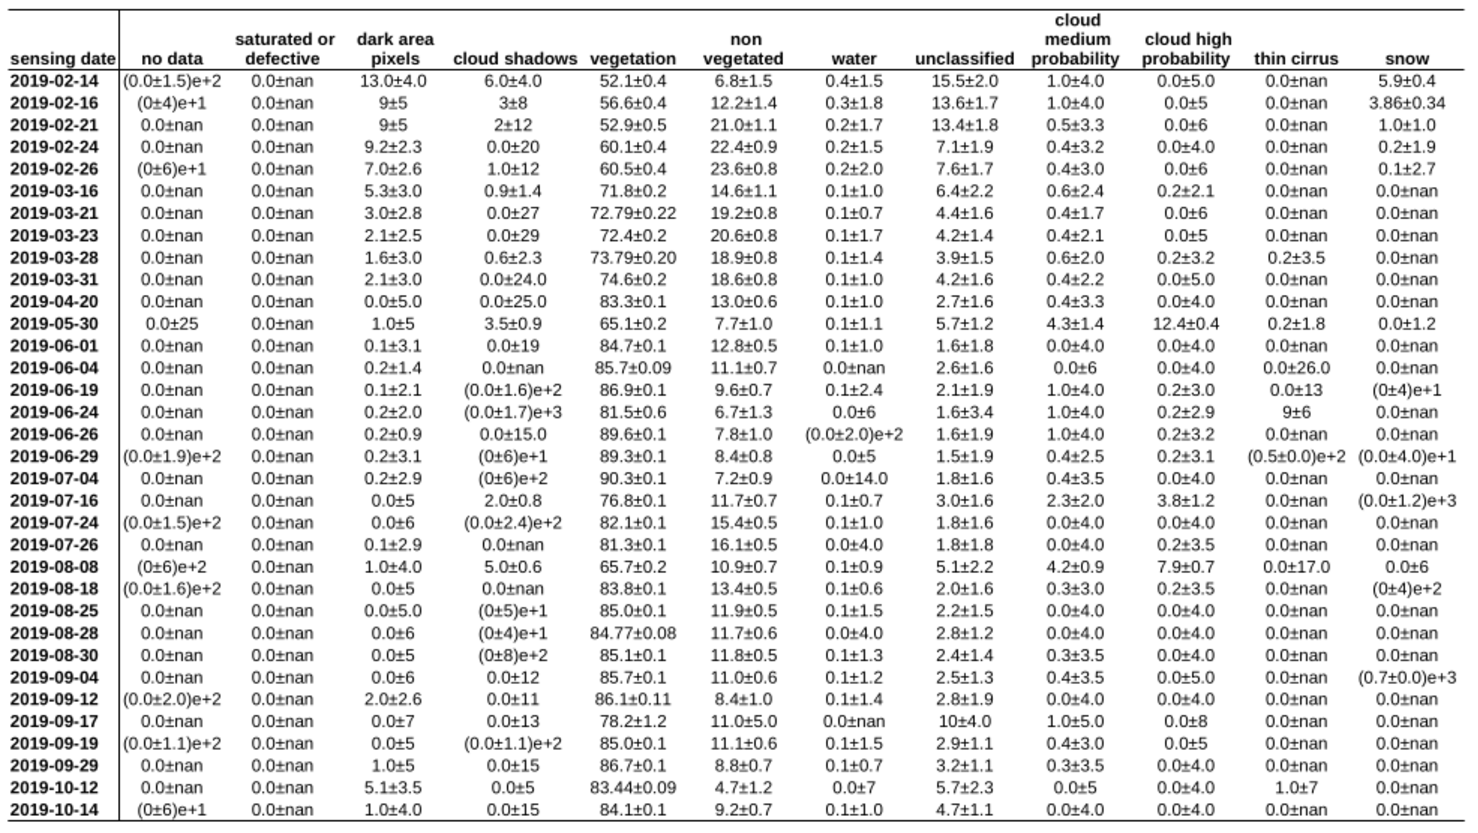
\includegraphics[width=\textwidth]{04-Uncertainty/img/SCL_Uncertainty_Table.pdf}
    \label{supp:scl_uncertainty}
\end{table}


\begin{figure}[H]
    \centering
    \includegraphics[width=\textwidth]{04-Uncertainty/img/Canola_all-pixels-uncertainty-timeseries.png}
    \caption{Spatio-temporal variability of EVI (left column), NDVI (mid column) and GLAI (right column) for all pixels annotated as rapeseed (70.4 ha). For each S2 scene, the median value (blue line), central 50\% (red) and 90\% spread (orange) across all pixels is shown not classified as cloud, shadow or snow based on the SCL data of the original S2 outputs after Sen2Cor. The top-row shows the spatial variability in the actual EVI, NDVI and GLAI derived from the S2 scenes. In the mid row, the absolute uncertainties derived from the MC simulations are depicted, whereas the bottom row shows the uncertainties in relative terms.}
    \label{fig:rapeseed-timeseries-and-uncertainty}
\end{figure}

\begin{figure}[H]
    \centering
    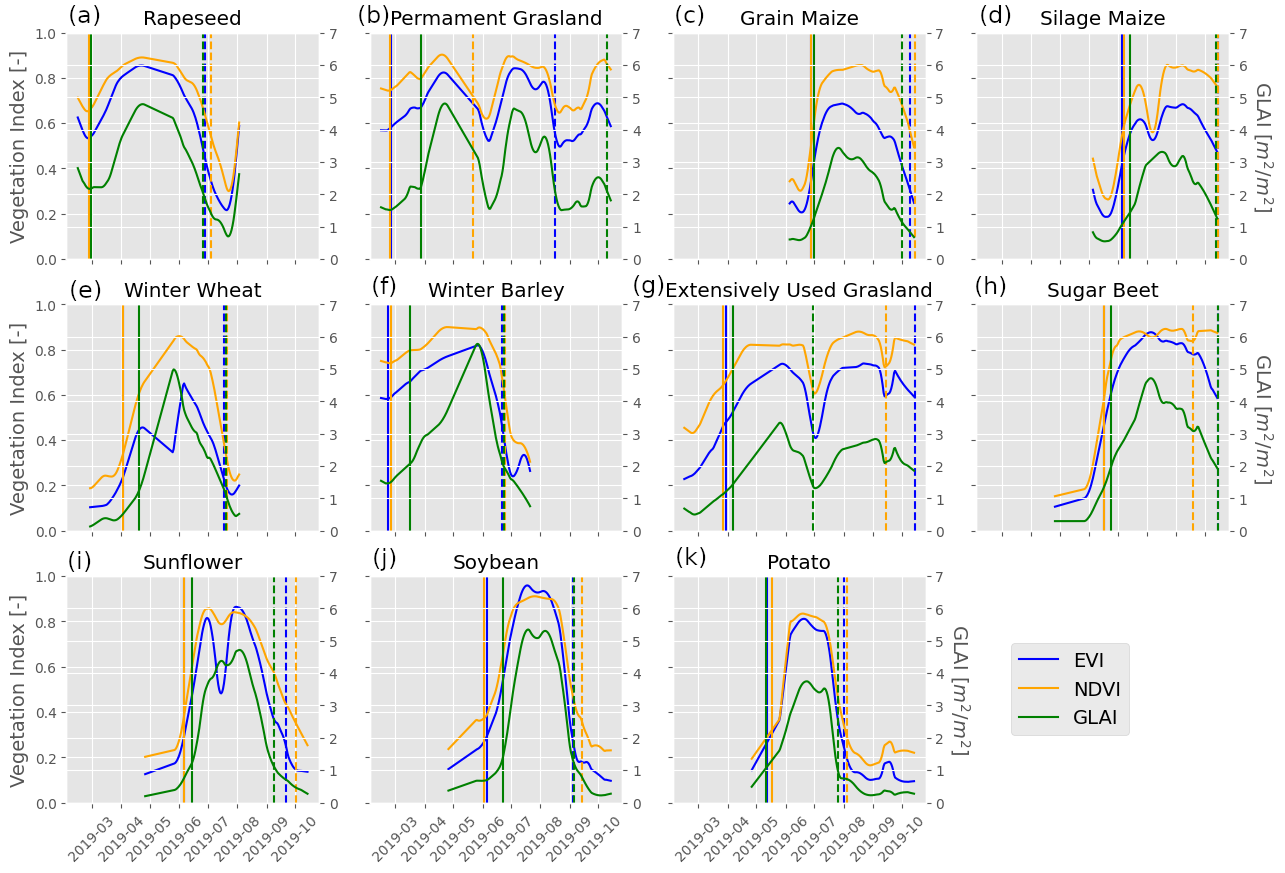
\includegraphics[width=\textwidth]{04-Uncertainty/img/130513_130438_sample_time_series.png}
    \caption{Sample time series of different crop types from randomly selected pixels showing EVI (blue), NDVI (orange) and GLAI (green). The curves have been outlier-filtered and interpolated to daily values using Savitzky-Golay.}
    \label{fig:sample_ts_pixels}
\end{figure}

\begin{figure}[H]
    \centering
    \includegraphics[width=\textwidth]{04-Uncertainty/img/Corn_all-pixels-uncertainty-timeseries.png}
    \caption{Spatio-temporal variability of EVI (left column), NDVI (mid column) and GLAI (right column) for all pixels annotated as grain maize (41.3 ha). For each S2 scene, the median value (blue line), central 50\% (red) and 90\% spread (orange) across all pixels is shown not classified as cloud, shadow or snow based on the SCL data of the original S2 outputs after Sen2Cor. The top-row shows the spatial variability in the actual EVI, NDVI and GLAI derived from the S2 scenes. In the mid row, the absolute uncertainties derived from the MC simulations are depicted, whereas the bottom row shows the uncertainties in relative terms.}
    \label{fig:grain-maize-timeseries-and-uncertainty}
\end{figure}

\begin{figure}[H]
    \centering
    \includegraphics[width=\textwidth]{04-Uncertainty/img/Extensively Used Grasland_all-pixels-uncertainty-timeseries.png}
    \caption{Spatio-temporal variability of EVI (left column), NDVI (mid column) and GLAI (right column) for all pixels annotated as extensively used grassland (62.9 ha). For each S2 scene, the median value (blue line), central 50\% (red) and 90\% spread (orange) across all pixels is shown not classified as cloud, shadow or snow based on the SCL data of the original S2 outputs after Sen2Cor. The top-row shows the spatial variability in the actual EVI, NDVI and GLAI derived from the S2 scenes. In the mid row, the absolute uncertainties derived from the MC simulations are depicted, whereas the bottom row shows the uncertainties in relative terms.}
    \label{fig:ext-used-grassland-timeseries-and-uncertainty}
\end{figure}

\begin{figure}[H]
    \centering
    \includegraphics[width=\textwidth]{04-Uncertainty/img/Permament Grasland_all-pixels-uncertainty-timeseries.png}
    \caption{Spatio-temporal variability of EVI (left column), NDVI (mid column) and GLAI (right column) for all pixels annotated as permanent grassland (168.9 ha). For each S2 scene, the median value (blue line), central 50\% (red) and 90\% spread (orange) across all pixels is shown not classified as cloud, shadow or snow based on the SCL data of the original S2 outputs after Sen2Cor. The top-row shows the spatial variability in the actual EVI, NDVI and GLAI derived from the S2 scenes. In the mid row, the absolute uncertainties derived from the MC simulations are depicted, whereas the bottom row shows the uncertainties in relative terms.}
    \label{fig:permanent-grassland-timeseries-and-uncertainty}
\end{figure}

\begin{figure}[H]
    \centering
    \includegraphics[width=\textwidth]{04-Uncertainty/img/Silage Maize_all-pixels-uncertainty-timeseries.png}
    \caption{Spatio-temporal variability of EVI (left column), NDVI (mid column) and GLAI (right column) for all pixels annotated as silage maize (175.6 ha). For each S2 scene, the median value (blue line), central 50\% (red) and 90\% spread (orange) across all pixels is shown not classified as cloud, shadow or snow based on the SCL data of the original S2 outputs after Sen2Cor. The top-row shows the spatial variability in the actual EVI, NDVI and GLAI derived from the S2 scenes. In the mid row, the absolute uncertainties derived from the MC simulations are depicted, whereas the bottom row shows the uncertainties in relative terms.}
    \label{fig:silage-maize-timeseries-and-uncertainty}
\end{figure}

\begin{figure}[H]
    \centering
    \includegraphics[width=\textwidth]{04-Uncertainty/img/Soybean_all-pixels-uncertainty-timeseries.png}
    \caption{Spatio-temporal variability of EVI (left column), NDVI (mid column) and GLAI (right column) for all pixels annotated as soybean (7.8 ha). For each S2 scene, the median value (blue line), central 50\% (red) and 90\% spread (orange) across all pixels is shown not classified as cloud, shadow or snow based on the SCL data of the original S2 outputs after Sen2Cor. The top-row shows the spatial variability in the actual EVI, NDVI and GLAI derived from the S2 scenes. In the mid row, the absolute uncertainties derived from the MC simulations are depicted, whereas the bottom row shows the uncertainties in relative terms.}
    \label{fig:soybean-timeseries-and-uncertainty}
\end{figure}

\begin{figure}[H]
    \centering
    \includegraphics[width=\textwidth]{04-Uncertainty/img/Sugar Beet_all-pixels-uncertainty-timeseries.png}
    \caption{Spatio-temporal variability of EVI (left column), NDVI (mid column) and GLAI (right column) for all pixels annotated as sugar beet (65.4 ha). For each S2 scene, the median value (blue line), central 50\% (red) and 90\% spread (orange) across all pixels is shown not classified as cloud, shadow or snow based on the SCL data of the original S2 outputs after Sen2Cor. The top-row shows the spatial variability in the actual EVI, NDVI and GLAI derived from the S2 scenes. In the mid row, the absolute uncertainties derived from the MC simulations are depicted, whereas the bottom row shows the uncertainties in relative terms.}
    \label{fig:sugar-beet-timeseries-and-uncertainty}
\end{figure}

\begin{figure}[H]
    \centering
    \includegraphics[width=\textwidth]{04-Uncertainty/img/Sunflower_all-pixels-uncertainty-timeseries.png}
    \caption{Spatio-temporal variability of EVI (left column), NDVI (mid column) and GLAI (right column) for all pixels annotated as sunflower (7.9 ha). For each S2 scene, the median value (blue line), central 50\% (red) and 90\% spread (orange) across all pixels is shown not classified as cloud, shadow or snow based on the SCL data of the original S2 outputs after Sen2Cor. The top-row shows the spatial variability in the actual EVI, NDVI and GLAI derived from the S2 scenes. In the mid row, the absolute uncertainties derived from the MC simulations are depicted, whereas the bottom row shows the uncertainties in relative terms.}
    \label{fig:sunflower-timeseries-and-uncertainty}
\end{figure}

\begin{figure}[H]
    \centering
    \includegraphics[width=\textwidth]{04-Uncertainty/img/Winter Barley_all-pixels-uncertainty-timeseries.png}
    \caption{Spatio-temporal variability of EVI (left column), NDVI (mid column) and GLAI (right column) for all pixels annotated as winter barley (63.4 ha). For each S2 scene, the median value (blue line), central 50\% (red) and 90\% spread (orange) across all pixels is shown not classified as cloud, shadow or snow based on the SCL data of the original S2 outputs after Sen2Cor. The top-row shows the spatial variability in the actual EVI, NDVI and GLAI derived from the S2 scenes. In the mid row, the absolute uncertainties derived from the MC simulations are depicted, whereas the bottom row shows the uncertainties in relative terms.}
    \label{fig:winter-barley-timeseries-and-uncertainty}
\end{figure}

\begin{figure}[H]
    \centering
    \includegraphics[width=\textwidth]{04-Uncertainty/img/Potato_all-pixels-uncertainty-timeseries.png}
    \caption{Spatio-temporal variability of EVI (left column), NDVI (mid column) and GLAI (right column) for all pixels annotated as potato (4.7 ha). For each S2 scene, the median value (blue line), central 50\% (red) and 90\% spread (orange) across all pixels is shown not classified as cloud, shadow or snow based on the SCL data of the original S2 outputs after Sen2Cor. The top-row shows the spatial variability in the actual EVI, NDVI and GLAI derived from the S2 scenes. In the mid row, the absolute uncertainties derived from the MC simulations are depicted, whereas the bottom row shows the uncertainties in relative terms.}
    \label{fig:potato-timeseries-and-uncertainty}
\end{figure}
